\documentclass[12pt,a4paper]{article}
\usepackage{hyperref}

\title{} 
\author{Simone Balducci, Gregorio Berselli}
\date{}

\usepackage{amsmath}
\usepackage{amsfonts}
\usepackage{amssymb}
\usepackage{amsthm}
\usepackage{braket}
\usepackage[margin=3cm]{geometry}
\usepackage{pgfplots}
\pgfplotsset{compat=1.18}
\usepackage{fancyhdr}
\usepackage{physics}
\usepackage{systeme,mathtools}
\usepackage{graphicx}
\usepackage{float}
\usepackage{relsize}
\usepackage{calligra}
\usepackage{siunitx}
\usepackage[miktex]{gnuplottex}
\usepackage{epstopdf}
\usepackage[english]{babel}
\usepackage{float}
\usepackage{tikz}
\usetikzlibrary{shapes.misc}
\usepackage[style=ieee]{biblatex}
\addbibresource{biblio.bib}

\newcommand{\R}{\Re}
\newcommand{\la}{\lambda}
\newcommand{\al}{\alpha}
\newcommand{\bd}{\textbf}
\newcommand{\lang}{\left\langle}
\newcommand{\rang}{\right\rangle}
\newcommand{\lbra}{\left\lbrace}
\newcommand{\rbra}{\right\rbrace}

\begin{document}

\maketitle

\begin{abstract}
    
\end{abstract}

\tableofcontents
\pagebreak

\section{Introduction}
One of the main challenge in the study of complex systems is to work out models that simplify real life problems giving likely solutions.
For this reason, years ago a new branch of physics was born, the so-called \emph{econophysics}.
The econophysics name first emerged with Stanley et al. at a conference held in 1995 in Kolkata.
It is a neologism used for the branch of physics of complex systems that seeks to make a complete survey of the statistical properties of financial markets, using the huge volume of data now available and working methods of statistical physics.
The goal is to understand economic phenomena through the application of physical models. \\
At the beginning of the twentieth century, Louis Bachelier (1870-1940) in his doctoral thesis in mathematics (\emph{Theory de La Speculation}, published in 1900), admitted that the prices of financial assets followed a random walk, anticipating the ideas from Einstein in five years on the mathematical formalization of a random walk process \cite{history}.
Years later, another paper signed by Fischer Black and Myron Scholes showed an application of the heat diffusion equation to financial problems. \\
Mandelbrot \cite{mandelbrot1965} also realized that normal distributions could not explain the high fluctuations in the price of cotton (using data from half a century), given that a distribution using the power law format fits the data better.  
However, he encountered the problem of infinite standard deviation: all moments of order greater than two were infinite.
The main problem is that in the financial markets the standard deviation is a measure of the volatility of a variable, i.e. its degree of variation over time, so it was difficult to give meaning to this greatness in case it becomes infinite.
An explanation came when Vilfredo Pareto (1848-1923), who was interested in the distribution of income in Italy in 1906, worked out Pareto's Power Law, justifying the results of Mandelbrot as fluctuations in assets.
Power laws have the property of being free of scale, so they are ideal for measuring phenomena that are susceptible to extreme events such as financial markets.
In fact, econophysics was intrinsically linked to seeking extreme events in financial series using power laws to describe them, and those events are not so rare (see 1987 and 2008 crisis).

The idea of this work is to test the ``fairness'' of money exchanges looking at the wealth distribution, using an agent-based model which code is available on GitHub at (\url{https://github.com/SimonB00/WealthDistributionModel}).
We tried to keep the model as simple as possible, making several tests varying the number of parameters according to their compatibility with real data.
Therefore, our study will start from a simple money exchange model on a fully connected network (with uniform probability) with an insight on a partial connected random network.
Then, a \emph{preferential attachment} will be implemented, trying to get better results.
For last, we introduce an ulterior ``saving parameter'' to see how this will influence the simulation.


\section{Fair Game hypothesis}
We want our model to be initially as simple as possible and then complicate it if necessary.
Let's consider $n$ agents with $\alpha$ coins each and let's define a time step as an interaction between two of them.
As interaction, we mean a match between two agents in which a cross-head game is played and the loser has to pay one coin to the winner.
In this case, we consider the probability to win equal to the probability to lose, regardless to the personal capital.
As boundary condition we assume that an agent will play only if he has at least 1 coin, effectively excluding those who have no money at all.
It's trivial that the ``0 state'' of this system is an attractor and the dynamics will tend to take all agents to 0 but one to $N = \alpha n$.
However, if we study the system at a sufficiently large time (but not so much to end up in the limit) we may find a well-defined trend.

In the fair game hypothesis every microstate has the same probability: our problem reduces to compute how many microstate corresponds to a unique macrostate.
How can we count the microstates?
For simplicity let's take 3 agents with one coin each: we can count the microstates of this system on the surface of a 3D simplex with sides of length 3, as shown in Fig. \ref{fig:threeSimplex}.
\begin{figure}[ht!]
    \centering
    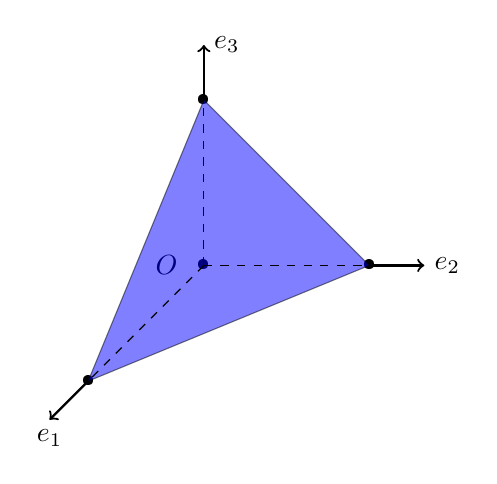
\begin{tikzpicture}[scale = .7]
        \tikzstyle{point}=[thick,draw=black,inner sep=0pt,minimum width=4pt,minimum height=4pt]

        \node (o)[label={[label distance=0cm]180:$O$}] at (0,0) {\textbullet};
        \node (a)[label={[label distance=0cm]0:}] at (3,0) {\textbullet};
        \node (b)[label={[label distance=0cm]0:}] at (0,3) {\textbullet};
        \node (c)[label={[label distance=0cm]270:}] at (-2.1, -2.1) {\textbullet};
        
        \draw[fill=blue, opacity=0.5] (a.center) -- (b.center) -- (c.center) -- cycle;
        \draw[dashed] (o.center) -- (a.center);
        \draw[dashed] (o.center) -- (b.center);
        \draw[dashed] (o.center) -- (c.center);

        \draw[thick, ->] (3,0) -- (4,0) node[anchor=west]{$e_2$};
        \draw[thick, ->] (0,3) -- (0,4) node[anchor=west]{$e_3$};
        \draw[thick, ->] (-2.1, -2.1) -- (-2.8, -2.8) node[anchor=north]{$e_1$};
    \end{tikzpicture}
    \caption{\emph{A 3D simplex where the surface of interest is enlightened.}}
    \label{fig:threeSimplex}
\end{figure}
It is clear that, while the surface gives us the number of microstates corresponding to a fixed amount of money, the volume between 0 and a fixed value $y$ such that $0 \leq y \leq N$ gives us the cumulative distribution of the microstates, Fig. (\ref{fig:simplexVolume}).
Defining our simplex as
\begin{equation*}
    \Delta^n(N)=\left\{x \in \mathbb{R}^n \text{ s.t. } \sum_{i = 1}^n x_i = N, x_i \geq 0\right\}
\end{equation*}
we can use the result of an article \cite{simplexSampling} in which the volume of a simplex between 0 and $y$ is found as
\begin{equation}
    V_n\left(y, N\right) = \frac{\sqrt{n+1}}{n!}\left[N^n - \left(N - y\right)^n\right]
\end{equation}
\begin{figure}[ht!]
    \centering
    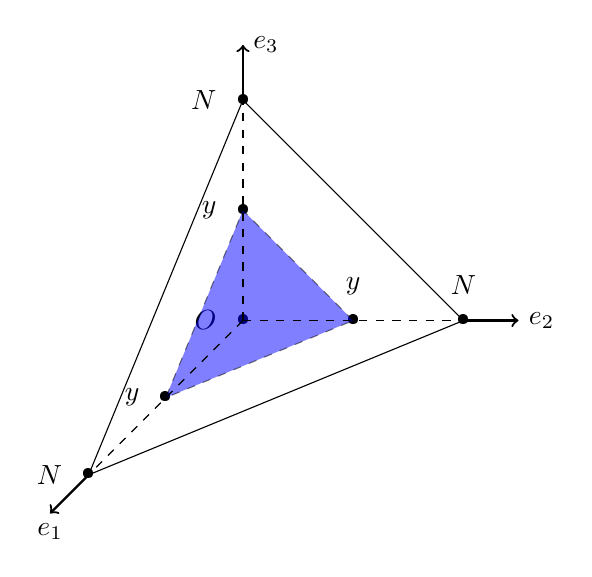
\begin{tikzpicture}[scale = .7]
        \tikzstyle{point}=[thick,draw=black,inner sep=0pt,minimum width=4pt,minimum height=4pt]

        \node (o)[label={[label distance=0cm]180:$O$}] at (0,0) {\textbullet};
        \node (a)[label={[label distance=0cm]90:$y$}] at (2,0) {\textbullet};
        \node (b)[label={[label distance=0cm]180:$y$}] at (0,2) {\textbullet};
        \node (c)[label={[label distance=0cm]180:$y$}] at (-1.4, -1.4) {\textbullet};

        \node (d)[label={[label distance=0cm]90:$N$}] at (4,0) {\textbullet};
        \node (e)[label={[label distance=0cm]180:$N$}] at (0,4) {\textbullet};    
        \node (f)[label={[label distance=0cm]180:$N$}] at (-2.8,-2.8) {\textbullet};  
        
        \draw[dashed, fill=blue, opacity=0.5] (a.center) -- (b.center) -- (c.center) -- cycle;
        \draw[dashed] (o.center) -- (d.center);
        \draw[dashed] (o.center) -- (e.center);
        \draw[dashed] (o.center) -- (f.center);
        \draw (d.center) -- (e.center) -- (f.center) -- cycle;

        \draw[thick, ->] (4,0) -- (5,0) node[anchor=west]{$e_2$};
        \draw[thick, ->] (0,4) -- (0,5) node[anchor=west]{$e_3$};
        \draw[thick, ->] (-2.8, -2.8) -- (-3.5, -3.5) node[anchor=north]{$e_1$};
    \end{tikzpicture}
    \caption{\emph{Fraction of volume of the simplex we are interested.}}
    \label{fig:simplexVolume}
\end{figure}
We want to normalize it all as we are looking for a pdf, so we can divide $V_n\left(y, N\right)$ by $V_n\left(N, N\right)$ finding the cumulative distribution
\begin{equation}
    F(y) = \frac{V_n\left(y, N\right)}{V_n\left(N, N\right)} = 1 - \left(1 - \frac{y}{N}\right)^n
\end{equation}
We note that in our case $N=\alpha n$ so
\begin{equation*}
    F(y) =  1 - \left[\left(1 - \frac{y}{\alpha n}\right)^{\alpha n}\right]^\frac{1}{\alpha}
\end{equation*}
but $n$ is the dimension of the simplex, i.e. the number of agents of the system itself.
For a great amount of agents we can take the previous relation in the limit $n\to\infty$ obtaining
\begin{equation}
    F(y) = 1 - e^{-\frac{y}{\alpha}}
\end{equation}
Now that we have the cumulative distribution of the microstate it's trivial to find the pdf applying the definition
\begin{equation*}
    f(y) = \frac{d}{dy}F(y) = \frac{1}{\alpha} e^{-\frac{y}{\alpha}}
\end{equation*}
Since we are only interested in the trend of the pdf, the result obtained can be synthesized into
\begin{equation}
    f(y) \propto e^{-\frac{y}{\alpha}}
\end{equation}


\subsection{Class permanence with a random network}

\section{Unfair Game hypothesis}

\section{Conclusions}

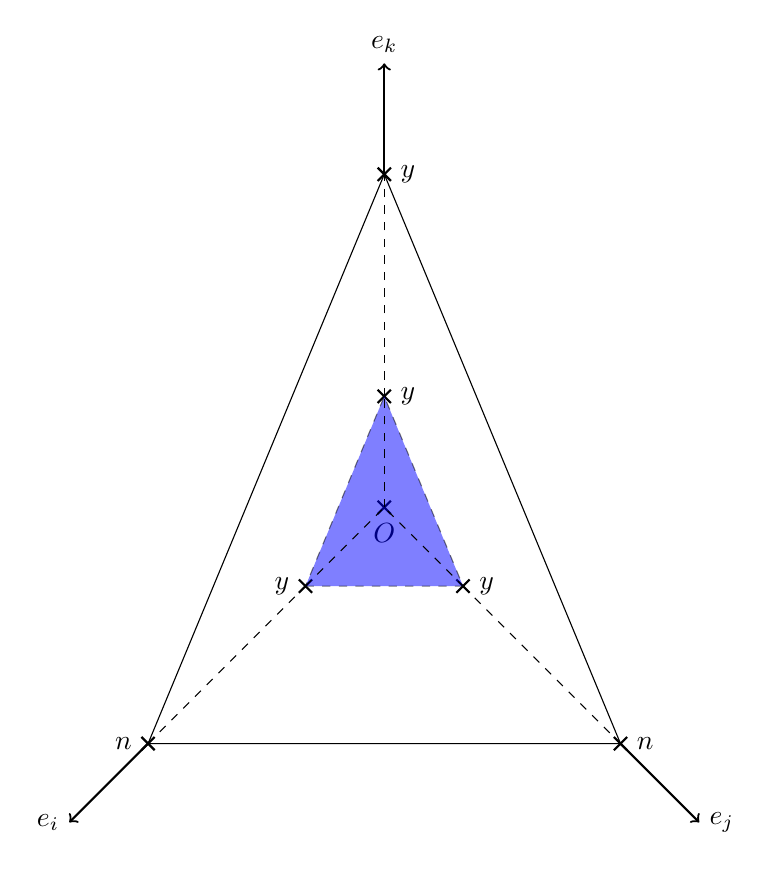
\begin{tikzpicture}
    \tikzstyle{point}=[thick,draw=black,cross out,inner sep=0pt,minimum width=4pt,minimum height=4pt]

    \node (a)[point,label={[label distance=0cm]180:$y$}] at (0,0) {};
    \node (b)[point,label={[label distance=0cm]0:$y$}] at (2,0) {};
    \node (c)[point,label={[label distance=0cm]0:$y$}] at (1,2.41) {};
    \node (d)[point,label={[label distance=0cm]270:$O$}] at (1,1) {};
    \node (e)[point,label={[label distance=0cm]180:$n$}] at (-2,-2) {};
    \node (f)[point,label={[label distance=0cm]0:$n$}] at (4,-2) {};
    \node (g)[point,label={[label distance=0cm]0:$y$}] at (1,5.23) {};
    \draw[dashed, fill=blue, opacity=0.5] (a.center) -- (b.center) -- (c.center) -- cycle;
    \draw (e.center) -- (f.center) -- (g.center) -- cycle;
    \draw[dashed] (e.center) -- (a.center);
    \draw[dashed] (b.center) -- (f.center);
    \draw[dashed] (c.center) -- (g.center);
    \draw[dashed] (a.center) -- (d.center) -- (b.center);
    \draw[dashed] (d.center) -- (c.center);

    \draw[thick, ->] (-2,-2) -- (-3,-3) node[anchor=east]{$e_i$};
    \draw[thick, ->] (4,-2) -- (5,-3) node[anchor=west]{$e_j$};
    \draw[thick, ->] (1,5.23) -- (1,6.64) node[anchor=south]{$e_k$};

\end{tikzpicture}

\printbibliography

\end{document}
